\chapter{统计结果}\label{chap:statistics}
在此搜寻中,并没有发现明显信号,所以构建以下似然函数比作为假设检验量。
\[ \tilde q_\mu = \left\{
  \begin{array}{l l}
    -2 \ln \frac{\mathcal{L}(\mu,\hat{\hat{\theta}}(\mu))}{\mathcal{L}(0,\hat{\hat{\theta}}(0))} & \quad \text{if $\hat\mu < 0$}\\
    -2 \ln \frac{\mathcal{L}(\mu,\hat{\hat{\theta}}(\mu))}{\mathcal{L}(\hat{\mu},\hat{\theta})} & \quad \text{if $0 \leq \hat\mu \leq \mu$}\\
    0 & \quad \text{if $\hat\mu > \mu$}
  \end{array} \right.\]
\noindent 其中$\hat{\theta}$ 表示无条件拟合,$\hat{\hat{\theta}}$ 表示有条件拟合 (即$\mu$ 为固定值). 利用此假设检验量,在渐近近似分布~\cite{Cowan:2010js}下基于
CL$_s$方法~\cite{Read:2002hq}即可得到产生截面上限。
\begin{itemize}
  \item 在95\% CL$_s$置信度下,标准模型希格斯对($pp\rightarrow hh$)观测(期望)产生截面上限为5.6 pb(4.8 pb),即168倍(145倍)标准模型预测值。
  \item 在95\% CL$_s$置信度下,共振态希格斯对($pp\rightarrow X \rightarrow hh$)的产生截面上限如表~\ref{tab:upper_limits_2lss}所示,对应图~\ref{fig:limit_plots_2lss}。
  \item 在95\% CL$_s$置信度下,$SS$($pp\rightarrow X\rightarrow SS$)随$m_S$或$m_X$变化的产生截面上限如表~\ref{tab:limits_HSS_combined}和图~\ref{fig:limit_HSS}所示。
\end{itemize}

\begin{table}[!ht]
\scriptsize
\begin{center}
\begin{tabular}{l|c|cccccccc}
\hline
\hline
             & SM Higgs pair & 260 GeV  & 300 GeV & 400 GeV &500 GeV   \\
\hline
Median &144.96 &36.96 &30.06 &12.09 &3.37 \\
Observed    &168.01 &31.53 &26.85 &11.72 &3.04 \\
\hline
$+2\sigma$ &292.48 &87.71 &66.75 &29.44 &7.18 \\
$+1\sigma$ &206.69 &56.13 &44.18 &18.33 &4.89 \\
$-1\sigma$ &104.45 &26.63 &21.66 &8.71 &2.43 \\
$-2\sigma$ &77.80 &19.84 &16.14 &6.49 &1.81 \\
\hline
\hline
\end{tabular}
\caption{The combined exclusion limits at the 95$\%$ $CL$ for the production cross section of a gluon fusion produced X boson times its branching ratio to hh.}
\label{tab:upper_limits_2lss}
\end{center}
\end{table}

\begin{figure}[!h!tpb]
  \centering
  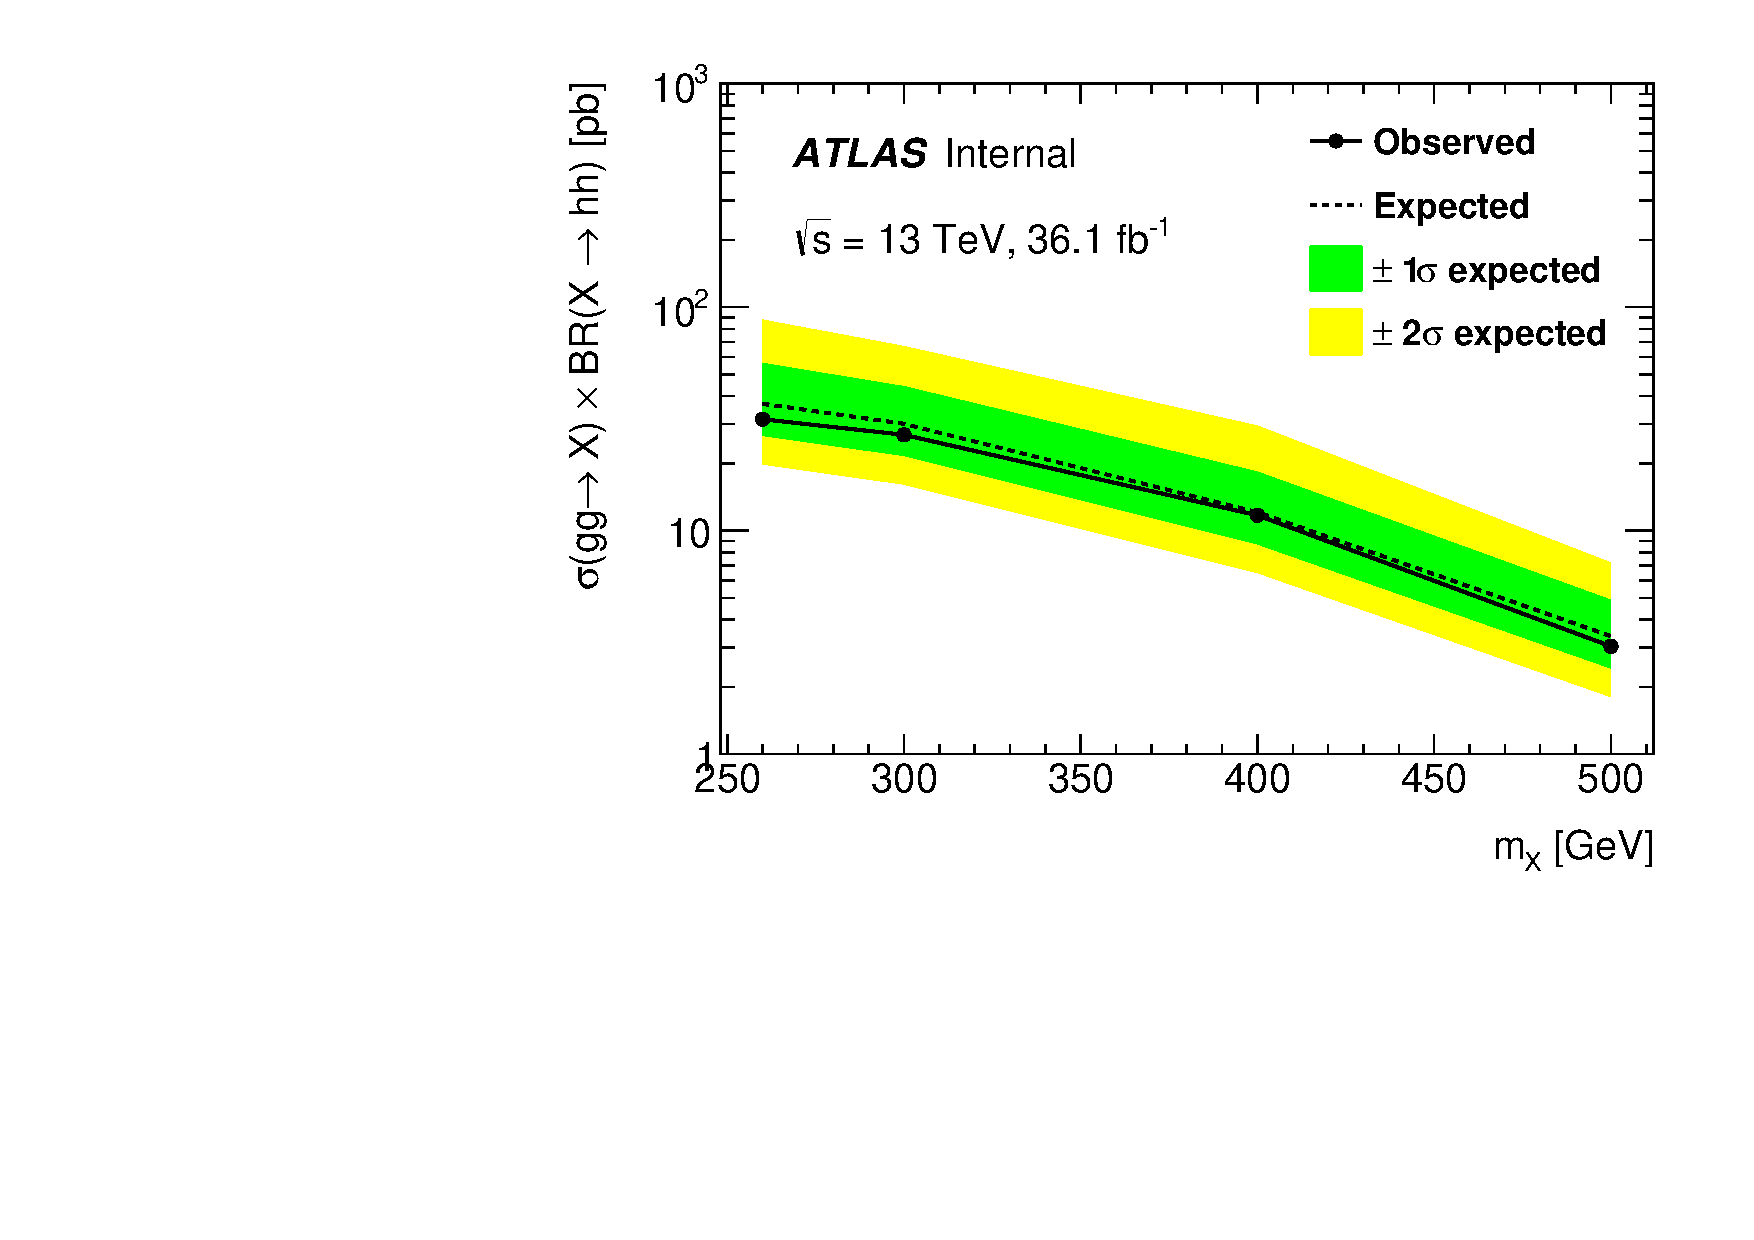
\includegraphics[width=0.55\textwidth, angle=-90]{fig/Statistical/limitAllSys.pdf}
  \caption{  The expected limits for $pp\rightarrow X \rightarrow hh$, as a function of mX.}
\label{fig:limit_plots_2lss}
\end{figure}

\begin{table}[h]
\scriptsize
\begin{center}
\begin{tabular}{cccccccccc}
\hline
\hline
& X280, S135 &X300, S135 &X320, S135 &X340, S135 &X340, S145  &X340, S155 &X340, S165 \\
\hline
Median &6.07 &5.68 &5.91 &4.85 &1.50 &0.69 &0.37 \\
Observed &4.85 &4.55 &4.75 &5.02 &1.47 &0.68 &0.38 \\
\hline
$+2\sigma$ &11.28 &10.15 &10.86 &8.98 &2.80 &1.31 &0.68 \\
$+1\sigma$ &8.24 &7.60 &8.01 &6.58 &2.03 &0.95 &0.50 \\
$-1\sigma$ &4.38 &4.09 &4.26 &3.50 &1.08 &0.50 &0.27 \\
$-2\sigma$ &3.26 &3.05 &3.17 &2.60 &0.80 &0.37 &0.20 \\
\hline
\hline
\end{tabular}
\caption{The combined exclusion limits at the 95$\%$ $CL$ for the production cross section of a gluon fusion produced X boson times its branching ratio to SS.}
\label{tab:limits_HSS_combined}
\end{center}
\end{table}
\begin{figure}[!h!tpb]
  \centering
  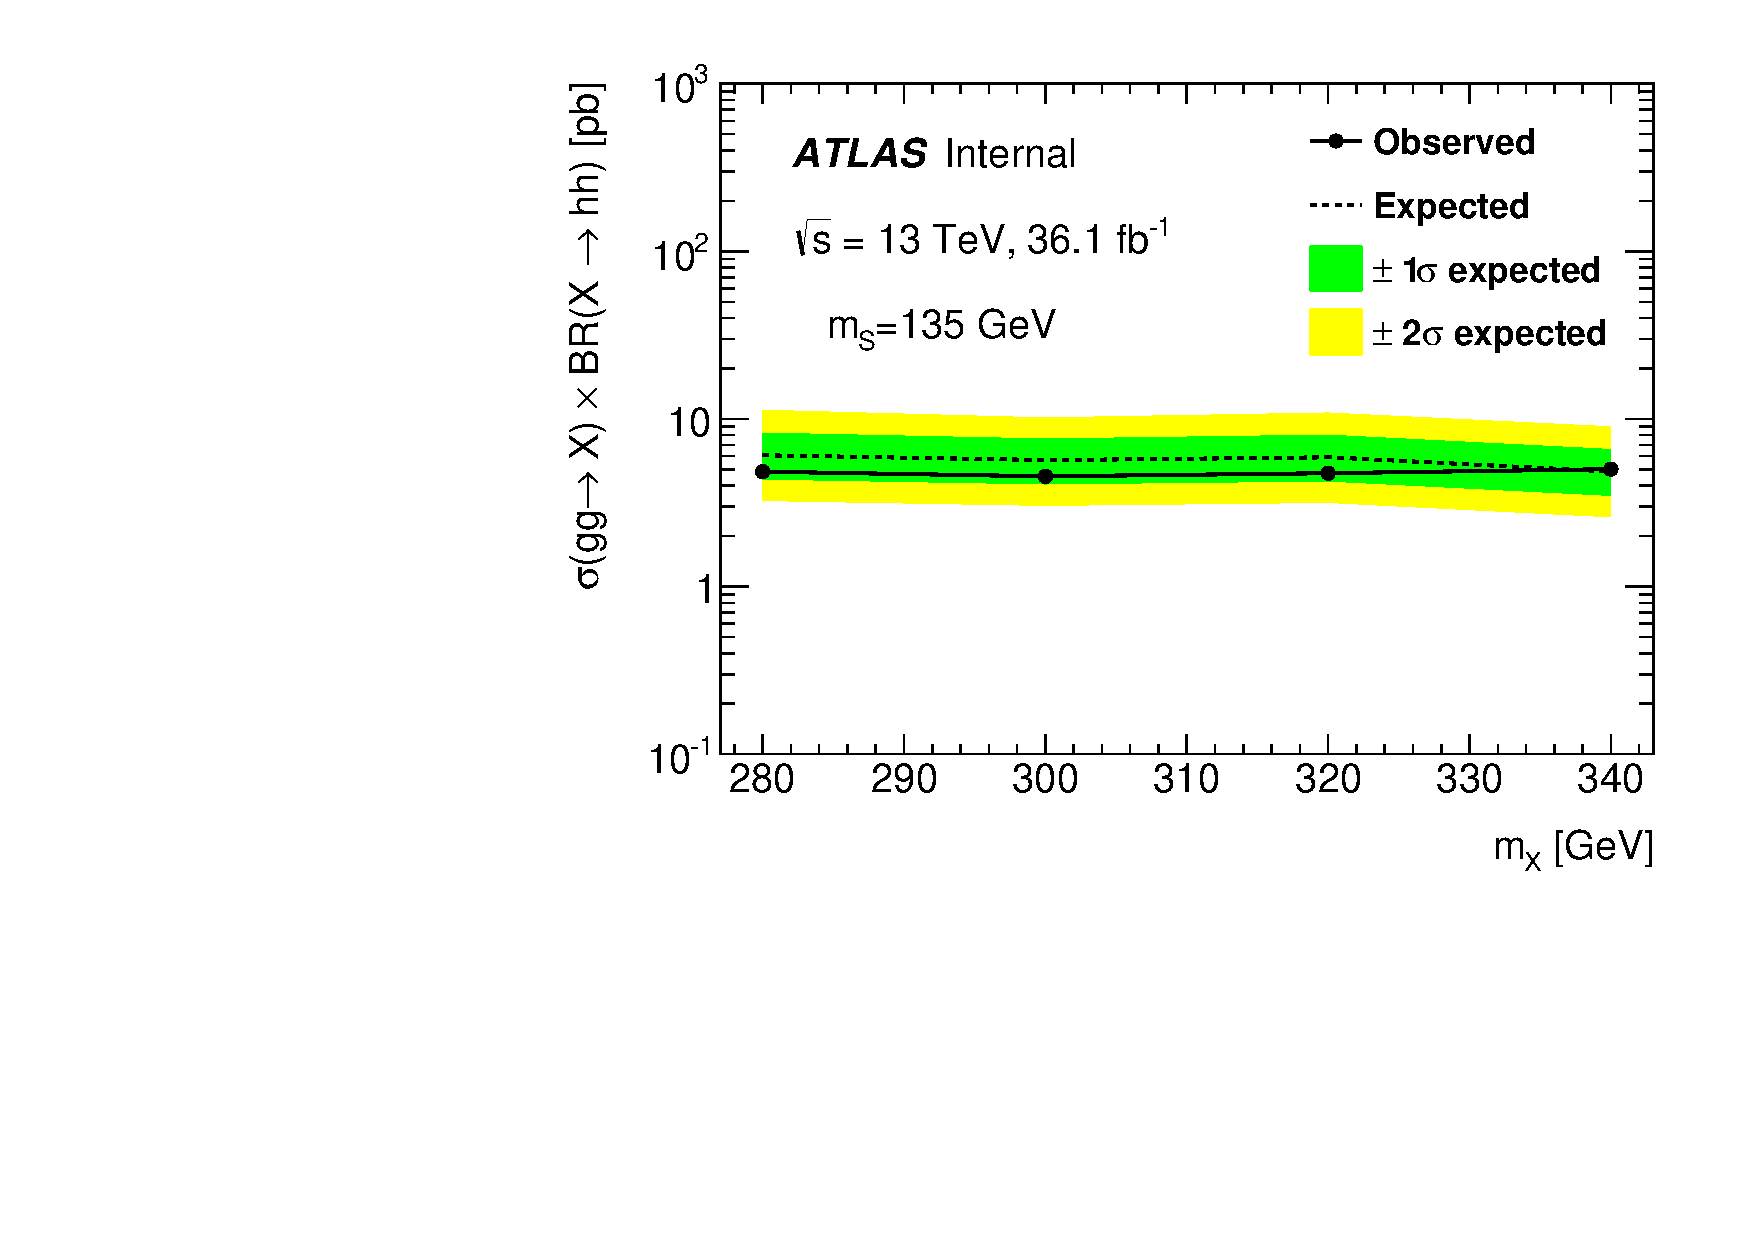
\includegraphics[width=0.35\textwidth, angle=-90]{fig/Statistical/limit_HSS_S135_AllSys.pdf}
  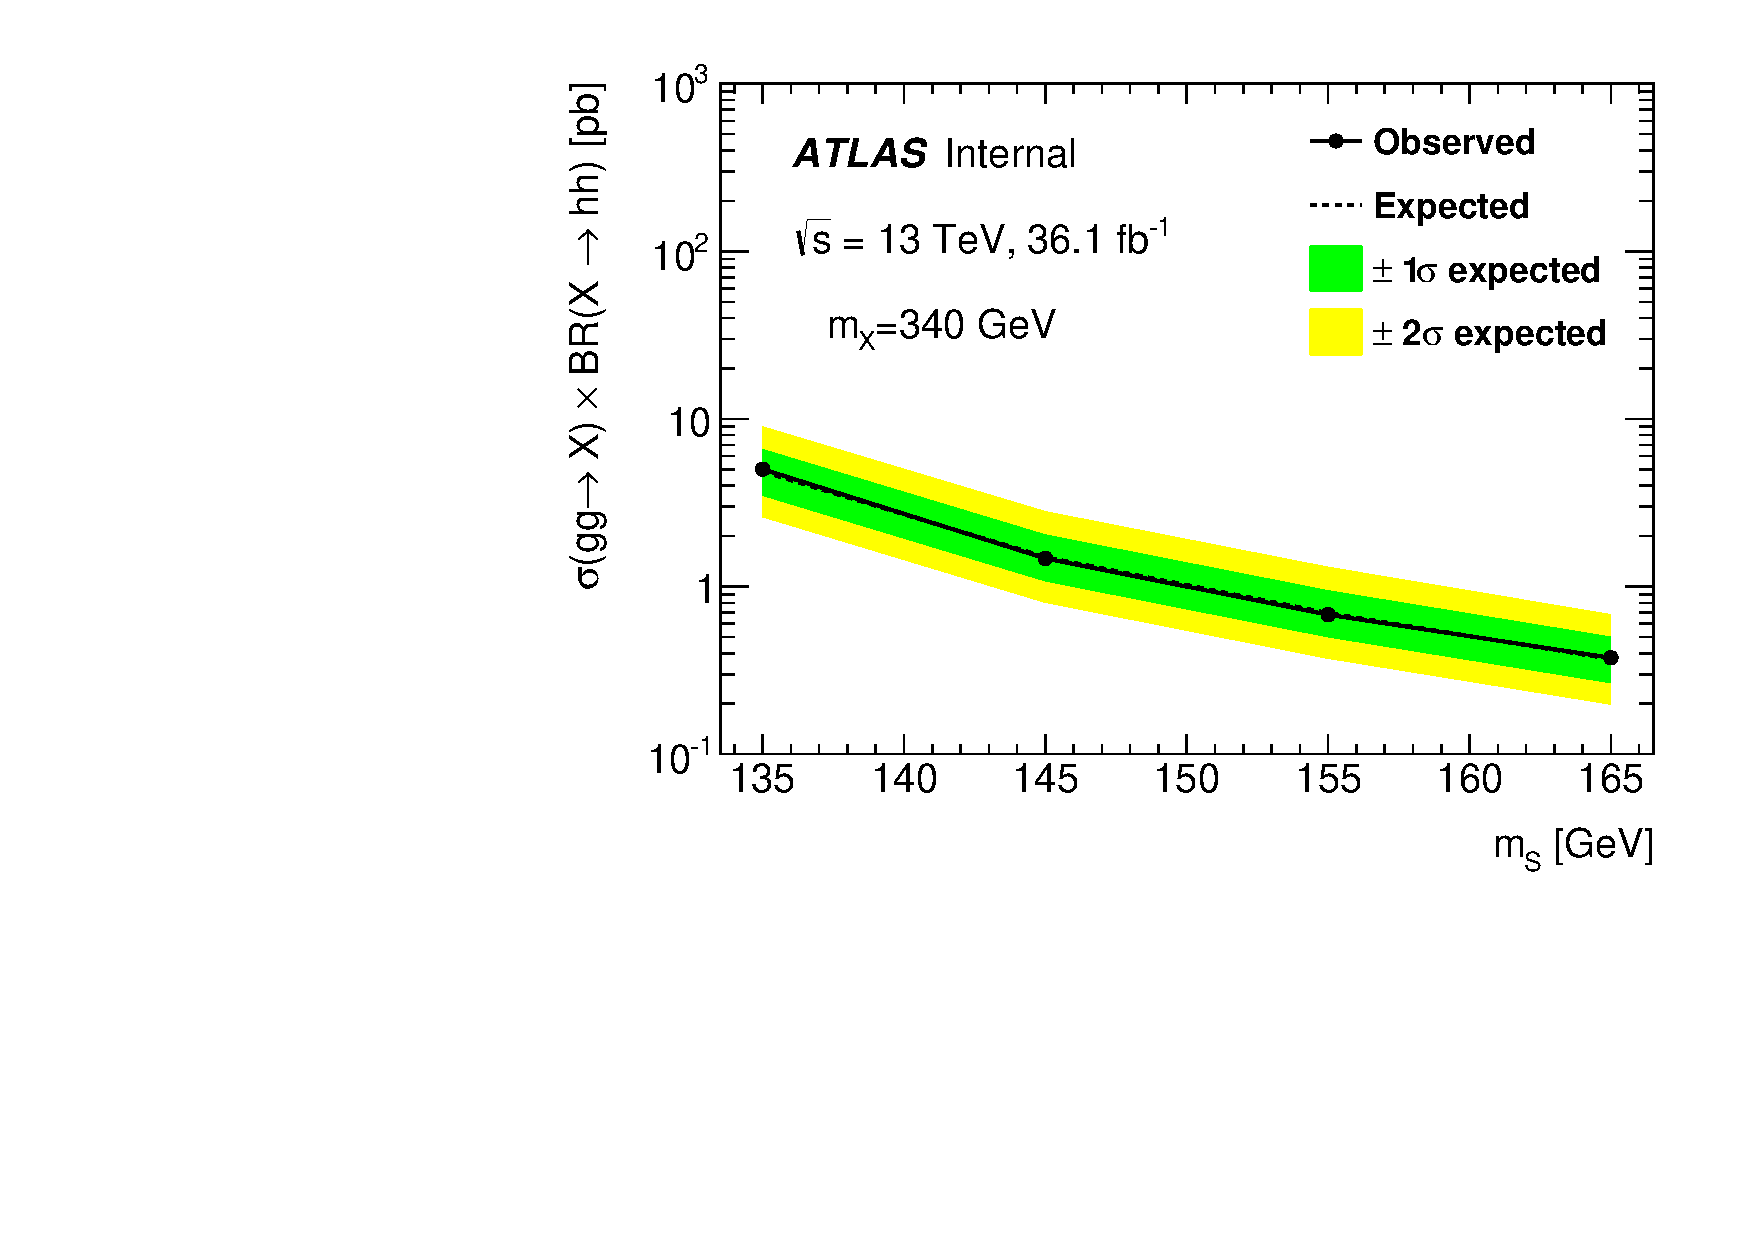
\includegraphics[width=0.35\textwidth, angle=-90]{fig/Statistical/limit_HSS_H340_AllSys.pdf}
  \caption{The expected limits for $pp\rightarrow X \rightarrow SS$ production. Left: fixing $m_S$=135~GeV; right: fixing $m_X$=340~GeV.}
\label{fig:limit_HSS}
\end{figure}